%% LyX 2.1.2 created this file.  For more info, see http://www.lyx.org/.
%% Do not edit unless you really know what you are doing.
\documentclass[14pt,english]{extarticle}
\usepackage[T1]{fontenc}
\usepackage[latin9]{inputenc}
\usepackage[letterpaper]{geometry}
\geometry{verbose,tmargin=0.1in,lmargin=0.7in,rmargin=0.7in,headheight=0.5in,headsep=0.5in}
\pagestyle{empty}
\usepackage{pifont}
\usepackage{amsmath}
\usepackage{graphicx}

\makeatletter
\@ifundefined{date}{}{\date{}}
\AtBeginDocument{
  \def\labelitemi{\ding{52}}
}

\makeatother

\usepackage{babel}
\begin{document}

\title{Completing Chemical Equations}


\author{(Example of Double Replacement Reaction)}

\maketitle
\vspace{-0.75in}


\thispagestyle{empty}
\enlargethispage{3\baselineskip}

\begin{align*}
\mathrm{ZnBr_{2}+NaCl\rightarrow}
\end{align*}


\vspace{-0.2in}


\begin{center}
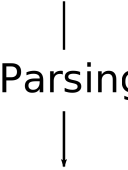
\includegraphics[scale=0.5]{arrow-parsing}
\par\end{center}

\vspace{-0.1in}


\texttt{Equation = {[}{[}{[}{[}``Zn'', 1{]}, {[}``Br'', 2{]}{]},
{[}{[}``Na'', 1{]}, {[}``Cl'', 1{]}{]}{]}, \_{]}}

\vspace{-0.1in}


\begin{center}
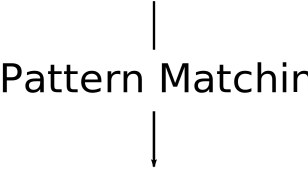
\includegraphics[scale=0.5]{arrow-pattern-matching}
\par\end{center}

\vspace{-0.5in}


\begin{flushleft}
\texttt{{[}{[}{[}Metal1,\_{]},{[}NonMetal1,\_{]}{]},{[}{[}Metal2,\_{]},{[}NonMetal2,\_{]}{]}{]},
{[}{[}{[}Metal1,\_{]},{[}NonMetal2,\_{]}{]},{[}{[}Metal2,\_{]},{[}NonMetal1,\_{]}{]}{]}} 
\par\end{flushleft}

\vspace{-0.2in}


\begin{center}
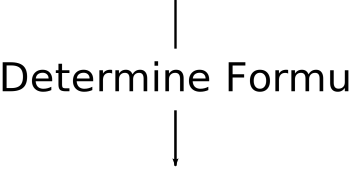
\includegraphics[scale=0.5]{arrow-det-formulas}
\par\end{center}

\vspace{-0.5in}


\begin{eqnarray*}
\mathrm{(Metal,ChargeM,NonMetal,ChargeNM)} & \Rightarrow & \mathrm{[[Metal,ChargeNM],[NonMetal,ChargeM]]}\\
\mathrm{("Na",1,"Br",-1)} & \Rightarrow & \mathrm{[["Na",1],["Br",1]]}\\
\mathrm{("Zn",2,"Cl",-1)} & \mathrm{\Rightarrow} & \mathrm{[["Zn",1],["Cl",2]]}
\end{eqnarray*}


\vspace{-0.2in}


\begin{center}
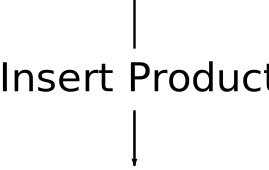
\includegraphics[scale=0.5]{arrow-ins-products}
\par\end{center}

\vspace{-0.3in}


\begin{flushleft}
\texttt{Equation = {[}{[}{[}{[}``Zn'', 1{]}, {[}``Br'', 2{]}{]},
{[}{[}``Na'', 1{]}, {[}``Cl'', 1{]}{]}{]}, {[}{[}{[}\textquotedbl{}Na\textquotedbl{},1{]},{[}\textquotedbl{}Br\textquotedbl{},1{]}{]},{[}{[}\textquotedbl{}Zn\textquotedbl{},1{]},{[}\textquotedbl{}Cl\textquotedbl{},2{]}{]}{]}{]}}
\par\end{flushleft}

\begin{center}
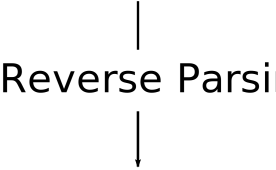
\includegraphics[scale=0.5]{arrow-deparsing}
\par\end{center}

\vspace{-0.5in}


\begin{align*}
\mathrm{ZnBr_{2}+NaCl} & \rightarrow\mathit{ZnCl_{2}+NaBr}
\end{align*}

\end{document}
